%%%%%%%%%%%%%%%%%%%%%%%%%%%%%%%%%%%%%%%%%
% Beamer Presentation
% LaTeX Template
% Version 1.0 (10/11/12)
%
% This template has been downloaded from:
% http://www.LaTeXTemplates.com
%
% License:
% CC BY-NC-SA 3.0 (http://creativecommons.org/licenses/by-nc-sa/3.0/)
%
%%%%%%%%%%%%%%%%%%%%%%%%%%%%%%%%%%%%%%%%%

%----------------------------------------------------------------------------------------
%	PACKAGES AND THEMES
%----------------------------------------------------------------------------------------

%\documentclass[UTF8,aspectratio=169,14pt]{ctexbeamer}
\documentclass[UTF8,aspectratio=169]{ctexbeamer}
\usepackage{hyperref}
\hypersetup{
	colorlinks=true,
	linkcolor=red,
	anchorcolor=blue,
	citecolor=green
}

\mode<presentation> {
	
	% The Beamer class comes with a number of default slide themes
	% which change the colors and layouts of slides. Below this is a list
	% of all the themes, uncomment each in turn to see what they look like.
	
	%\usetheme{default}
	%\usetheme{AnnArbor}
	%\usetheme{Antibes}
	%\usetheme{Bergen}
	%\usetheme{Berkeley}
	%\usetheme{Berlin}
	%\usetheme{Boadilla}
	%\usetheme{CambridgeUS}
	%\usetheme{Copenhagen}
	%\usetheme{Darmstadt}
	%\usetheme{Dresden}
	%\usetheme{Frankfurt}
	%\usetheme{Goettingen}
	%\usetheme{Hannover}
	%\usetheme{Ilmenau}
	%\usetheme{JuanLesPins}
	%\usetheme{Luebeck}
	\usetheme{Madrid}
	%\usetheme{Malmoe}
	%\usetheme{Marburg}
	%\usetheme{Montpellier}
	%\usetheme{PaloAlto}
	%\usetheme{Pittsburgh}
	%\usetheme{Rochester}
	%\usetheme{Singapore}
	%\usetheme{Szeged}
	%\usetheme{Warsaw}
	
	% As well as themes, the Beamer class has a number of color themes
	% for any slide theme. Uncomment each of these in turn to see how it
	% changes the colors of your current slide theme.
	
	%\usecolortheme{albatross}
	%\usecolortheme{beaver}
	%\usecolortheme{beetle}
	%\usecolortheme{crane}
	%\usecolortheme{dolphin}
	%\usecolortheme{dove}
	%\usecolortheme{fly}
	%\usecolortheme{lily}
	%\usecolortheme{orchid}
	%\usecolortheme{rose}
	%\usecolortheme{seagull}
	%\usecolortheme{seahorse}
	%\usecolortheme{whale}
	%\usecolortheme{wolverine}
	
	%\setbeamertemplate{footline} % To remove the footer line in all slides uncomment this line
	%\setbeamertemplate{footline}[page number] % To replace the footer line in all slides with a simple slide count uncomment this line
	
	%\setbeamertemplate{navigation symbols}{} % To remove the navigation symbols from the bottom of all slides uncomment this line
}

\usepackage{graphicx} % Allows including images
\graphicspath{{./figs/}}
\usepackage{booktabs} % Allows the use of \toprule, \midrule and \bottomrule in tables
\usepackage{longtable}
\usepackage{listings}
\usepackage{xcolor}
\lstset{numbers=left, %设置行号位置
	numberstyle=\tiny, %设置行号大小
	keywordstyle=\color{blue}, %设置关键字颜色
	commentstyle=\color[cmyk]{1,0,1,0}, %设置注释颜色
	frame=single, %设置边框格式
	escapeinside=``, %逃逸字符(1左面的键),用于显示中文
	%breaklines, %自动折行
	extendedchars=false, %解决代码跨页时,章节标题,页眉等汉字不显示的问题
	xleftmargin=2em,xrightmargin=2em, aboveskip=1em, %设置边距
	tabsize=4, %设置tab空格数
	showspaces=false %不显示空格
}
% Fonts
% \usepackage{libertine}
% \setmonofont{Courier}
\setCJKsansfont[ItalicFont=Noto Serif CJK SC Black, BoldFont=Noto Sans CJK SC Black]{Noto Sans CJK SC}
\setmainfont[Ligatures={Common,TeX}]{Linux  Libertine O}
\setmonofont[SmallCapsFont={Latin Modern Mono Caps}]{Latin Modern Mono Light}
\setsansfont{Linux Biolinum O}

\logo{
\includegraphics[width=0.55cm,height=0.55cm]{../../thcs-logo.png}}

%----------------------------------------------------------------------------------------
%	TITLE PAGE
%----------------------------------------------------------------------------------------

\title[第14讲]{第14讲: Concurrency in OS Kernel} % The short title appears at the bottom of every slide, the full title is only on the title page
\subtitle{第一节:Introduction}
\author{陈渝} % Your name
\institute[清华大学] % Your institution as it will appear on the bottom of every slide, may be shorthand to save space
{
	清华大学计算机系 \\ % Your institution for the title page
	\medskip
	\textit{yuchen@tsinghua.edu.cn} % Your email address
}
\date{\today} % Date, can be changed to a custom dateC++ memory order



\begin{document}

\begin{frame}
\titlepage % Print the title page as the first slide
\end{frame}
    
%\begin{frame}
%\frametitle{提纲} % Table of contents slide, comment this block out to remove it
%\tableofcontents % Throughout your presentation, if you choose to use \section{} and \subsection{} commands, these will automatically be printed on this slide as an overview of your presentation
%\end{frame}
%
%%----------------------------------------------------------------------------------------
%%	PRESENTATION SLIDES
%%----------------------------------------------------------------------------------------
%

%----------------------------------------------
%-------------------------------------------------
\begin{frame}
    \frametitle{Resource}
    
    
    

	\begin{columns}
    
    \begin{column}{.5\textwidth}
        \centering
        
        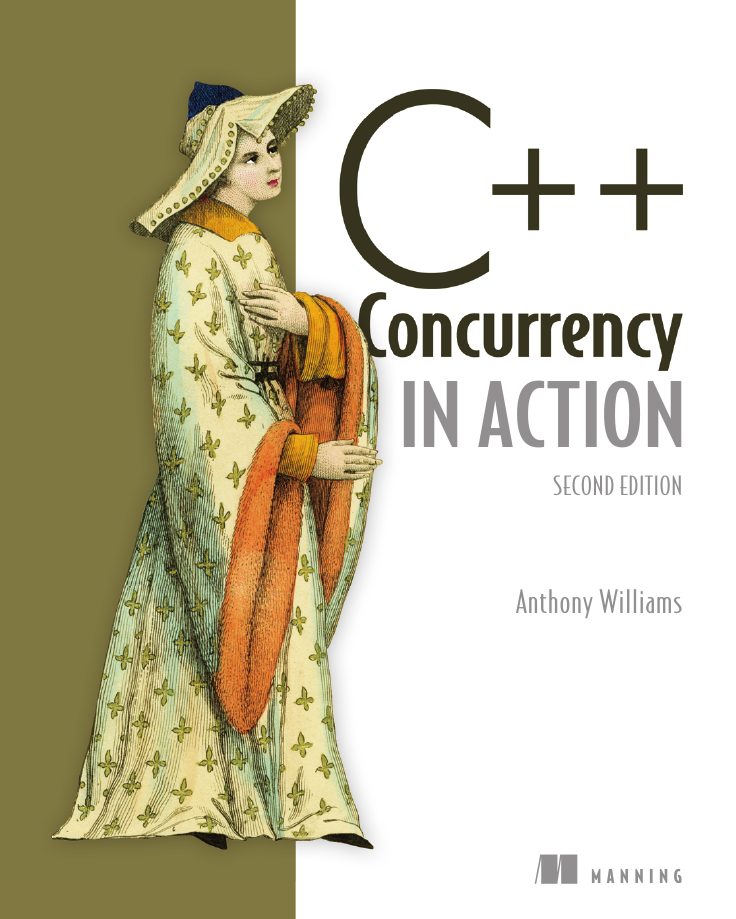
\includegraphics[width=.7\textwidth]{book-cpp-concurrency-in-action}
        
    \end{column}
    
    \begin{column}{.5\textwidth}
        
      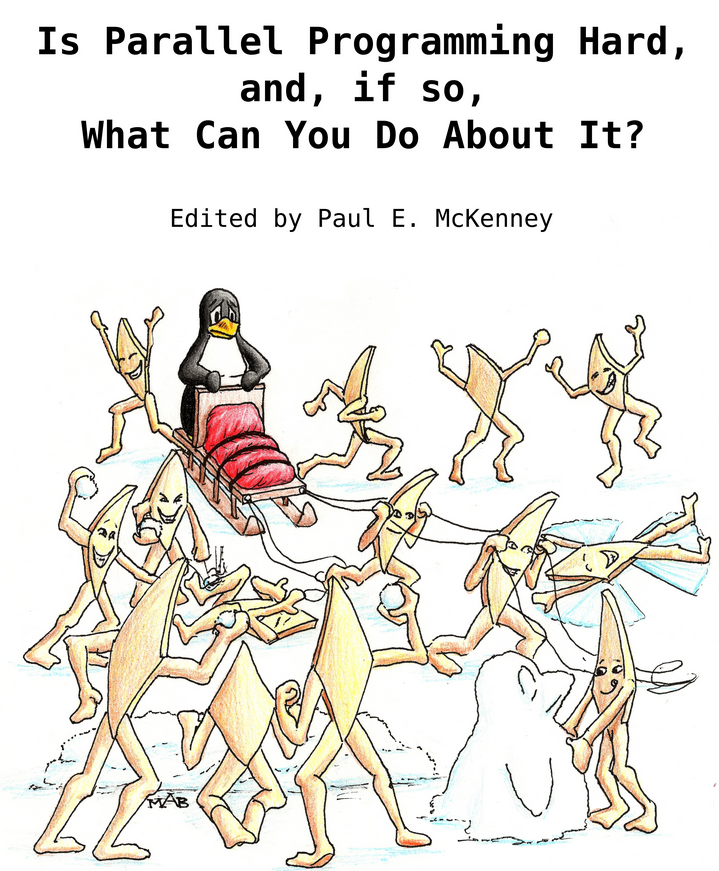
\includegraphics[width=.7\textwidth]{perfbook}
       
        
    \end{column}
    
    
\end{columns}
    
    \tiny Reference:
    
    "Is Parallel Programming Hard, And, If So, What Can You Do About It?",Paul McKenney;\\
    "C++Concurrency in Action", ANTHONY WILLIAMS; \\
    "CS510 - Advanced Topics in Concurrency", Jonathan Walpole 
\end{frame}

%----------------------------------------------
\begin{frame}[fragile]
    \frametitle{Locking In The Linux Kernel}
    \Large
    \begin{itemize}
    \item Why do we need locking in the kernel?
    \item Which problems are we trying to solve?
    \item What implementation choices do we have?
    \item Is there a one-size-fits-all solution?
  
\end{itemize}
    
\end{frame}


%----------------------------------------------
\begin{frame}[fragile]
    \frametitle{Concurrency in Linux}
    \Large
    \begin{itemize}
        \item Linux is a symmetric multiprocessing (SMP)
        preemptible kernel
        
        \item Its has true concurrency
        
        \item And various forms of pseudo concurrency
        
        
    \end{itemize}
    
\end{frame}


%----------------------------------------------
\begin{frame}[fragile]
    \frametitle{Sources of Pseudo Concurrency in Linux}
    \Large
    Software-based preemption
    \begin{itemize}
        \item Voluntary preemption (sleep/yield)
        \item  Involuntary preemption (preemptable kernel)
        \item And various forms of pseudo concurrency
        \item Solutions: don't do the former, disable preemption to
        prevent the latter
               
    \end{itemize}
    
\end{frame}


%----------------------------------------------
\begin{frame}[fragile]
    \frametitle{Sources of Pseudo Concurrency in Linux}
    \Large
    Hardware preemption
    \begin{itemize}
        \item Interrupt/trap/fault/exception handlers can start
        executing at any time       
        \item Solutions: disable interrupts
    \end{itemize}
    
\end{frame}


%----------------------------------------------
\begin{frame}[fragile]
    \frametitle{Uniprocessor Example
    }
    %    \normalsize
    \large    
    \begin{block}{}
        \begin{verbatim}
    preempt disable;
        r1 = x;
        r2 = x;
    preempt enable;
    assert (r1 == r2)
    \end{verbatim}
    \end{block}
    
\end{frame}

%----------------------------------------------
\begin{frame}[fragile]
    \frametitle{Uniprocessor Example
    }
    %    \normalsize
    \large    
    \begin{block}{}
        \begin{verbatim}
    preempt disable;
        r1 = x;
        yield();
        r2 = x;
    preempt enable;
    assert (r1 == r2)
    \end{verbatim}
    \end{block}    
\end{frame}


%----------------------------------------------
\begin{frame}[fragile]
    \frametitle{Uniprocessor Example
    }
    %    \normalsize
    \large    
    \begin{block}{}
        \begin{verbatim}
    interrupt disable;
        r1 = x;
        r2 = x;
    interrupt enable;
    assert (r1 == r2)
        \end{verbatim}
    \end{block}    
\end{frame}

%----------------------------------------------
\begin{frame}[fragile]
    \frametitle{True Concurrency in Linux}
    \Large
    Solutions to pseudo-concurrency do not work in the presence of
    true concurrency
    
    Alternatives include atomic operators, various forms of locking,
    RCU, and non-blocking synchronization
    
    Locking can be used to provide mutually exclusive access to
    critical sections
    \normalsize
    \begin{itemize}
        \item Locking can not be used everywhere, i.e., interrupt handlers
        can't block
               
        \item  Locking primitives must support coexistence with various
        solutions for pseudo concurrency, i.e., we need hybrid
        primitives
        
    \end{itemize}
    
\end{frame}


%----------------------------------------------
\begin{frame}[fragile]
    \frametitle{Multiprocessor Example}
    %    \normalsize
    \large    
    \begin{block}{}
        \begin{verbatim}
    interrupt disable;
        r1 = x;
        r2 = x;
    interrupt enable;
    assert (r1 == r2)
        \end{verbatim}
    \end{block}    
\end{frame}


%----------------------------------------------
\begin{frame}[fragile]
    \frametitle{Atomic Operators in Linux}
    \Large
    Simplest synchronization primitives
    \normalsize
    \begin{itemize}
        \item Primitive operations that are indivisible
    \end{itemize}
    \Large
    Two types
    \normalsize
\begin{itemize}
    \item methods that operate on integers
    \item  methods that operate on bits
\end{itemize}    

    \Large
Implementation

\normalsize
\begin{itemize}
    \item Assembly language sequences that use the atomic read-
    modify-write instructions of the underlying CPU
    architecture
    
\end{itemize}

\end{frame}


%----------------------------------------------
\begin{frame}[fragile]
    \frametitle{Memory Invariance Example  }
    %    \normalsize
    \large    
    \begin{block}{}
        \begin{verbatim}
        r1 = atomic read x;
        r2 = atomic read x;
        assert (r1 == r2)
        \end{verbatim}
    \end{block}    
\end{frame}


%----------------------------------------------
\begin{frame}[fragile]
    \frametitle{Atomic Integer Operators }
    %    \normalsize
    \large    
    \begin{block}{}
        \begin{verbatim}
    atomic_t v;
    atomic_set(&v, 5); /* v = 5 (atomically) */
    atomic_add(3, &v); /* v = v + 3 (atomically) */
    atomic_dec(&v);    /* v = v - 1 (atomically) */
    
    printf("This will print 7: %d\n", atomic_read(&v));
        \end{verbatim}
    \end{block}    
 "atomic\_add(3,\&v);"  is NOT the same as "atomic\_add(1,\&v); atomic\_add(2,\&v);"
 
\end{frame}


%----------------------------------------------
\begin{frame}[fragile]
    \frametitle{Spin Locks in Linux}
    \Large
    Mutual exclusion for larger (than one operator)
    critical sections requires additional support
    
    Spin locks are one possibility
    \normalsize
    \begin{itemize}
        \item Single holder locks
        \item When lock is unavailable, the acquiring process
        keeps trying
    \end{itemize}    
\end{frame}

%----------------------------------------------
\begin{frame}[fragile]
    \frametitle{Basic Use of Spin Locks  }
    \large    
\begin{block}{}
    \begin{verbatim}
    spinlock_t mr_lock = SPIN_LOCK_UNLOCKED;
    spin_lock(&mr_lock);
    /* critical section ... */
    spin_unlock(&mr_lock);
\end{verbatim}
\end{block}        
    
    \Large
    spin\_lock()
%    \normalsize
    \begin{itemize}
        \item Acquires the spinlock using atomic instructions required
        for SMP
    \end{itemize}    
    spin\_unlock()
%    \normalsize
\begin{itemize}
    \item Releases the spinlock
\end{itemize} 

\end{frame}


%----------------------------------------------
\begin{frame}[fragile]
    \frametitle{Spin Locks and Interrupts}
    \Large
    Interrupting a spin lock holder may cause problems
%    \normalsize
    \begin{itemize}
        \item  Spin lock holder is delayed, so is every thread
        spin waiting for the spin lock
        \item Not a big problem if interrupt handlers are short
        \item Interrupt handler may access the data
        protected by the spin-lock

        \begin{itemize}
            \item Should the interrupt handler use the lock?
            \item Can it be delayed trying to acquire a spin lock?
            \item What if the lock is already held by the thread it interrupted?           
        \end{itemize}
    \end{itemize}    
\end{frame}

%----------------------------------------------
\begin{frame}[fragile]
    \frametitle{Solutions for Spin Locks and Interrupts}
    \Large

        \begin{itemize}
            \item Should the interrupt handler use the lock?
            \item Can it be delayed trying to acquire a spin lock?
            \item What if the lock is already held by the thread it interrupted?           
        \end{itemize}
    -----------------------------------------
    \begin{itemize}
        \item If data is only accessed in interrupt context and is local to one
        specific CPU we can use interrupt disabling to synchronize
        
        \item If data is accessed from other CPUs we need additional
        synchronization -- spin lock
        
        \item Normal code (kernel context) must disable interrupts and
        acquire spin lock
        
    \end{itemize}

\end{frame}


%----------------------------------------------
\begin{frame}[fragile]
    \frametitle{Spin Locks \& Interrupt Disabling}
    \large    
    \begin{block}{}
        \begin{verbatim}
    spinlock_t mr_lock = SPIN_LOCK_UNLOCKED;
    unsigned long flags;
    spin_lock_irqsave(&mr_lock, flags); /* critical section ... */
    spin_unlock_irqrestore(&mr_lock, flags);
\end{verbatim}
    \end{block}        
    
    \Large
    spin\_lockk\_irqsave()
    %    \normalsize
    \begin{itemize}
        \item Disables interrupts locally
        \item Acquires the spinlock using instructions required for SMP
    \end{itemize}    
    spin\_unlock\_irqrestore()
    %    \normalsize
    \begin{itemize}
        \item Restores interrupts to the state they were in when the
        lock was acquired\large
        \begin{itemize}
            \item Contention for semaphores causes blocking not spinning
            \item Should not be used for short duration critical sections!
            \item Can be used to synchronize with user contexts that
            might block or be preempted
        \end{itemize}  
    \end{itemize} 
    
\end{frame}


%----------------------------------------------
\begin{frame}[fragile]
    \frametitle{Bottom Halves and Softirqs}
    \Large
    Softirqs, tasklets and BHs are deferrable functions
    \large
    \begin{itemize}
       \item delayed interrupt handling work that is scheduled
       \item they can wait for a spin lock without holding up devices
       \item they can access non-CPU local data
    
    \end{itemize}
\Large
    Softirqs – the basic building block
    \large
    \begin{itemize}
        \item statically allocated and non-preemptively scheduled
\item  can not be interrupted by another softirq on the same CPU
\item can run concurrently on different CPUs, and synchronize with
each other using spin-locks
    \end{itemize}
\Large
    Bottom Halves
    \large
\begin{itemize}
    \item built on softirqs
    \item can not run concurrently on different CPUs
\end{itemize}
    
\end{frame}


%----------------------------------------------
\begin{frame}[fragile]
    \frametitle{Spin Locks \& Deferred Functions}
    \Large
    spin\_lock\_bh()
    
    \large
    \begin{itemize}
        \item Implements the standard spinlock
        \item Disables softirqs
        \item Allows the softirq to use non-preemption only
    \end{itemize}
    \Large
    spin\_unlock\_bh()
    \large
    \begin{itemize}
        \item Releases the spinlock
        \item Enables softirqs
    \end{itemize}

\end{frame}


%----------------------------------------------
\begin{frame}[fragile]
    \frametitle{Spin Lock Rules}
    \Large
        \begin{itemize}
        \item Do not try to re-acquire a spinlock you already hold!
        \item Spinlocks should not be held for a long time!
        \item Do not sleep while holding a spinlock!
        
    \end{itemize}

    
\end{frame}


%----------------------------------------------
\begin{frame}[fragile]
    \frametitle{Semaphores}
    \Large
    Semaphores are locks that are safe to hold for
    longer periods of time
    \large
    \begin{itemize}
        \item Contention for semaphores causes blocking not spinning
        \item Should not be used for short duration critical sections!
        \item Can be used to synchronize with user contexts that
        might block or be preempted
     \end{itemize}  
\end{frame} 
 
%----------------------------------------------
 \begin{frame}[fragile]
 \frametitle{Spin Locks \& Interrupt Disabling}
 \large    
 \begin{block}{}
     \begin{verbatim}
     spinlock_t mr_lock = SPIN_LOCK_UNLOCKED;
     unsigned long flags;
     spin_lock_irqsave(&mr_lock, flags); /* critical section ... */
     spin_unlock_irqrestore(&mr_lock, flags);
     \end{verbatim}
 \end{block} 
\end{frame}

%----------------------------------------------
\begin{frame}[fragile]
    \frametitle{Semaphore Implementation}
    \Large
    Implemented as a wait queue and a usage count
    
    \large
    \begin{itemize}
        \item wait queue: list of processes blocking on the semaphore
        
        \item usage count: number of concurrently allowed holders
        
    \end{itemize}  

    down()
    \begin{itemize}
        \item  Attempts to acquire the semaphore by decrementing the
        usage count and testing if it is negative
        \item Blocks if usage count is negative
   \end{itemize}  

    up()
\begin{itemize}
    \item  releases the semaphore by incrementing the usage count
    and waking up one or more tasks blocked on it
    
\end{itemize}  




\end{frame}


%----------------------------------------------
\begin{frame}[fragile]
    \frametitle{Semaphore Implementation}
    \Large
    Implemented as a wait queue and a usage count
    
    \large
    \begin{itemize}
        \item wait queue: list of processes blocking on the semaphore
        
        \item usage count: number of concurrently allowed holders
        
    \end{itemize}  
    
    down\_interruptible()
    
    \begin{itemize}
        \item  Returns –EINTR if signal received while blocked
        \item Returns 0 on success        
    \end{itemize}  
    
    down\_trylock()
    \begin{itemize}
        \item  Attempts to acquire the semaphore
        \item  On failure it returns nonzero instead of blocking
    \end{itemize}  
    
\end{frame}



%----------------------------------------------
\begin{frame}[fragile]
    \frametitle{Reader-Writer Locks }
    \Large
    No need to synchronize concurrent readers unless a
    writer is present \\
    
    
    Both spin locks and semaphores have reader/writer
    variants
\end{frame}


%----------------------------------------------
\begin{frame}[fragile]
    \frametitle{Reader-Writer Spin Locks}
    \large    
    \begin{block}{}
        \begin{verbatim}
rwlock_t mr_rwlock = RW_LOCK_UNLOCKED;

read_lock(&mr_rwlock);
/* critical section (read only) ... */
read_unlock(&mr_rwlock);

write_lock(&mr_rwlock);
/* critical section (read and write) ... */
write_unlock(&mr_rwlock);

        \end{verbatim}
    \end{block} 
\end{frame}

%----------------------------------------------
\begin{frame}[fragile]
    \frametitle{Reader-Writer Semaphores}
    \large    
    \begin{block}{}
        \begin{verbatim}
    struct rw_semaphore mr_rwsem;
    init_rwsem(&mr_rwsem);
    
    down_read(&mr_rwsem); /* critical region (read only) ... */
    up_read(&mr_rwsem);
    
    down_write(&mr_rwsem); /* critical region (read and write) ... */
    up_write(&mr_rwsem);
\end{verbatim}
    \end{block} 
\end{frame}


%----------------------------------------------
\begin{frame}[fragile]
    \frametitle{Conclusions}
    \Large    
Wow! Why does one system need so many different
ways of doing synchronization?
    \begin{itemize}
    \item  Actually, there are more ways to do synchronization in
    Linux, this is just “locking”!
\end{itemize}  
\end{frame}


%----------------------------------------------
\begin{frame}[fragile]
    \frametitle{Conclusions}
    \Large    
   One size does not fit all:
   
    \begin{itemize}
        \item  Need to be aware of different contexts in which code
        executes (user, kernel, interrupt etc) and the implications
        this has for whether hardware or software preemption or
        blocking can occur
        \item The cost of synchronization is important, particularly its
        impact on scalability
    \end{itemize}  
\end{frame}
\end{document}